In questo capitolo parleremo in maniera più approfondita del linguaggio Vadalog e di tutte le sue particolarità. \newline
Vadalog è un linguaggio che raggiunge un attento equilibrio tra espressività e complessità, e può essere utilizzato come reasoning core di un KGMS. Fa parte della famiglia Warded Datalog$^\pm$ un frammento della famiglia Datalog$^\pm$ descritta in precedenza. \newline 
Il capitolo è organizzato come segue, nella sezione 1.1 verrà descritto in maniera approfondita il core del linguaggio, che a sua volta è diviso in due sottosezione, la sezione 1.1.1 che descrive il core logico dei linguaggi Datalog$^\pm$, tutte le proprietà e i vincoli che esso induce, arricchito con degli esempi, la sezione 1.1.2 che descrive il core logico di Vadalog,: le proprietà della famiglia Warded Datalog$^\pm$, infine la sezione 1.1.3 descrive la complessità e le caratteristiche del linguaggio Vadalog.\newline
Nella sezione 1.2 è possibile trovare dei programmi Vadalog di esempio per permettere una maggiore comprensione del linguaggio.
Questo capitolo prende spunto da diversi articoli pubblicati dal gruppo VADA, sia per alcune nozioni teoriche che per esempi pratici descritti~\cite{bellomarini2017swift, gottlob2015beyond}.

\section{Il core del linguaggio}

Il linguaggio Vadalog, fa parte della famiglia di linguaggi Warded Datalog$^\pm$, che a sua volta rappresenta un frammento della famiglia di linguaggi Datalog$\pm$, ovvero una restrizione della famiglia Datalog$^\pm$, in particolare garantendone la decidibilità. \newline
In questa sezione andremo a focalizzarci proprio su tali famiglie di linguaggi e le relative complessità, sono presenti tre sezioni, una che descrive il core logico dei linguaggi appartenenti alla famiglia di linguaggi Datalog$^\pm$, una che descrive il core logico di Vadalog, e come soddisfa la decidibilità, infine è presente una sezione per descrivere la complessità del core logico Vadalog.

\subsection{Il core logico dei linguaggi Datalog$\pm$}

L'obiettivo principale dei linguaggi Datalog$\pm$ è quello di estendere il noto linguaggio Datalog con funzionalità di modellazione utili come quantificatori esistenziali nelle teste delle regole (il + nel simbolo $\pm $), e contemporaneamente limitare la sintassi della regola, in modo tale che sia garantita la decidibilità e la tracciabilità dei dati del reasoning (il - nel simbolo $\pm $). \newline
Il core dei linguaggi Datalog$\pm $ è costituito da regole note come regole esistenziali, che generalizzano le regole Datalog con quantificatori esistenziali nelle teste delle regole, un esempio di regola esistenziale: \[Person(x) \rightarrow \exists y ~HasFather(x,y), Person(y)\]
che esprime che ogni persona, ha un padre che anch'esso a sua volta è una persona. \newline
In generale, una regola esistenziale è una frase di primo ordine: \[\forall \bar{x} \forall \bar{y} (\phi(\bar{x}, \bar{y}) \rightarrow \exists \bar{z} \psi (\bar{x}, \bar{z})\]
dove $\phi$  ()il corpo) e $\psi$  (la testa) sono congiunzioni di atomi con costanti e variabili. \newline
La semantica di un insieme di regole esistenziali $\Sigma$ sopra un database D, chiamata $\Sigma$(D), è definita mediante una procedura. Durante questa procedura vengono aggiunti nuovi atomi a D (coinvolgendo anche valori nulli per soddisfare le variabili esistenziali), finché il risultato finale $\Sigma$(D) non soddisfa tutte le regole esistenziali (solitamente infinito). \newline
Vediamo un esempio di tale procedura: \newline
Consideriamo un Database D = {Person(Bob)}, e la regola esistenziale: \[Person(x) \rightarrow \exists y ~HasFather(x,y), Person(y)\]
L'atomo del database D innesca la regola esistenziale e vengono aggiunti i seguenti atomi: \[HasFather(Bob, \nu_{1}) ~e~ Person(\nu_{1})\]
$\nu_{1}$ è un labeled null che rappresenta un valore sconosciuto.\newline
Il nuovo atomo Person($\nu_{1}$) innesca nuovamente la regola esistenziale, e vengono aggiunti altri atomi a D: \[HasFather(\nu_{1}, \nu_{2}) ~e~ Person(\nu_{2})\]
Dove $\nu_{2}$ è un nuovo nullo. Il risultato è l'istanza: \[\{Person(Bob), HasFather(Bob, \nu_{1})\} \cup \underset{i>0}{\bigcup} ~\{Person(\nu_{i}), HasFather(\nu_{i}, \nu_{i+1})\}\]
$\nu_{1}$, $\nu_{2}$, ..., $\nu_{i}$, $\nu_{i+1}$ sono labeled nulls. \newline \newline
Data una coppia Q=($\Sigma$, Ans), dove $\Sigma$ è un insieme di variabili esistenziali e Ans un predicato n-ario, la valutazione di Q su un database D, indicata Q(D), è definita come set di tuple sopra sopra l'insieme $C_{d}$ di valori costanti che occorrono nel database D. \newline
Il compito principale del reasoning è l'inferenza di tuple: dato un database D, una coppia Q = ($\Sigma$, Ans), ed una tupla di costanti $\bar{t}$, bisogna decidere se $\bar{t}$ appartiene a Q. Questo problema è molto difficile, infatti è indecidibile, anche quando Q è fisso e solo D è dato come input~\cite{cali2013taming}. \newline
Ciò ha portato all'attività di identificare restrizioni sulle regole esistenziali che rendono tale problema decidibile. Ciascuna di queste restrizioni genera un nuovo linguaggio della famiglia Datalog$\pm$. \newline

\subsection{Il core logico di Vadalog}

Vadalog è un linguaggio logico e rappresenta un'estensione di Datalog, quindi un programma Vadalog è composto da un insieme di regole. \newline
In ogni regola è possibile trovare una testa ed un corpo, nel quale ogni testa è composta da un insieme di atomi, ed ogni corpo da un insieme di atomi e un insieme di condizioni. Gli atomi del corpo possono rappresentare: degli atomi di input (collegamento diretto ad unità di storage), presenti in teste di altre regole o nella regola stessa (ricorsione). \newline 
Ogni atomo può essere composto da un numero indefinito di argomenti, che possono essere variabili o costanti. \newline
Le condizioni sono di varia natura, possono rappresentare l'assegnazione di una variabile, una condizione booleana che si vuole verificare e tante altre possibilità implementate dal linguaggio Vadalog. \newline
Un esempio di regola contenente atomi composti da variabili e costanti: \[a(X) :- b(X,"Hi")\]
Poiché Vadalog appartiene alla famiglia di linguaggi Warded Datalog$^\pm$, contiene quantificatori esistenziali nelle teste generando valori nulli. \newline
Nel linguaggio Vadalog, ci sono tre tipologie di variabili che sono contraddistinte:

\begin{enumerate}
	\item Harmless: Variabili standard presenti nel corpo di una regola, che non possono assumere valori nulli.
	\item Harmful: Rappresentano dei nulli presenti nel corpo di una regola, e che sono a loro volta un quantificatore esistenziale nella testa di un'altra regola.
	\item Dangerous: Sono le variabili che rappresentano gli esiste nelle teste delle regole.
\end{enumerate}

Vadalog si basa sulla nozione di \emph{wardedness}, proprietà ereditata dalla famiglia di linguaggi Warded Datalog$^\pm$~\cite{gottlob2015beyond}. \newline
La wardedness applica una restrizione su come vengono utilizzate le variabili "\textit{dangerous}" (pericolose) di un insieme di regole esistenziali. Intuitivamente una variabile dangerous è una variabile del corpo che può essere unificata con un valore nullo quando viene applicato l'algoritmo di ricerca e viene propagato anche alla testa della regola.\newline
Per esempio dato l'insieme $\Sigma$ di regole esistenziali \[P(x) \rightarrow \exists z~R(x,z)~e~R(x,y) \rightarrow P(y)\]
La variabile y nel corpo della seconda regola è dangerous. Dato un database D = \{P(a)\}, l'algoritmo applica la prima regola e genera R(a, $\nu$), dove $\nu$ è un nullo che funge da testimone della variabile esistenziale \textit{z}, e poi la seconda regola verrà applicata con la variabile \textit{y} che è unificata con $\nu$ che viene propagata all'atomo ottenuto P($\nu$). \newline

\begin{figure}[h!]
	\centering
	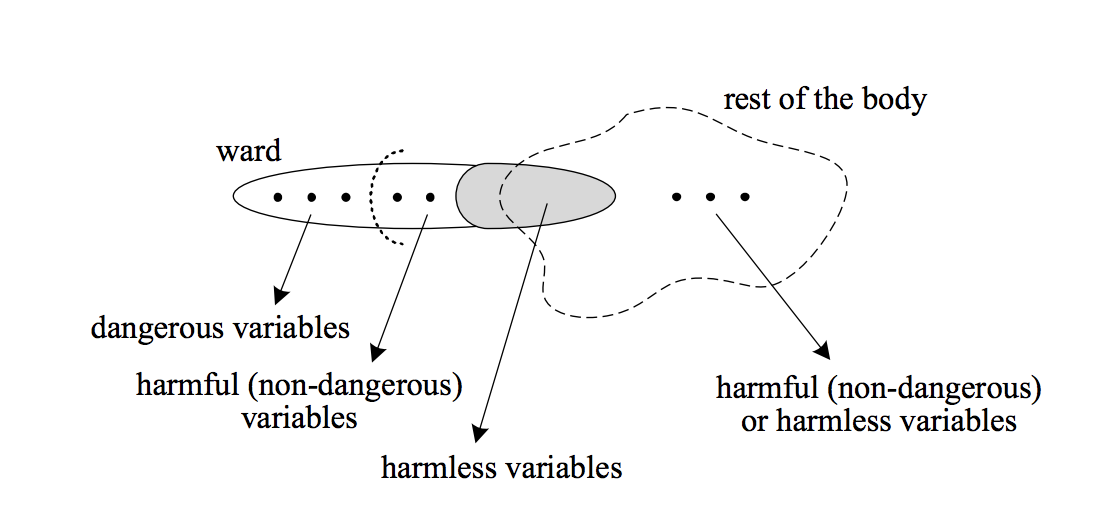
\includegraphics[width=0.8\linewidth]{figure/wardedness}
	\caption{Corpo di una regola warded~\cite{gottlob2015beyond}.}
	\label{fig:wardedness}
\end{figure}
L'obiettivo della wardedness è quello di verificare il modo in cui i valori nulli vengono propagati ponendo le seguenti condizioni: 
\begin{enumerate}
	\item  Tutte le variabili dangerous devono coesistere in un singolo corpo di un atomo A, chiamato il ward, e 
	\item Il ward può condividere solo variabili \textit{harmless} con il resto del corpo.
\end{enumerate}
Una regola è warded se vengono rispettate entrambe le condizioni appena citate, in Figura~\ref{fig:wardedness} possiamo vederne un esempio grafico. \newline

\subsection{Complessità}

In questa sezione viene descritta la complessità di Warded Datalog$^\pm$, anche facendo riferimenti a possibili frammenti di esso. \newline
Warded Datalog$\pm$ è composto da insiemi (finiti) di regole esistenziali warded, esso rappresenta una raffinatezza di \textit{Weakly-Frontier-Guarded Datalog$\pm$}, che è una famiglia di linguaggi definita allo stesso modo ma senza la condizione 2 sopra citata~\cite{baget2011rules}.
Weakly-Frontier-Guarded Datalog$\pm$ è intrattabile nella complessità dei dati, infatti è EXPTIME-completo. \newline \newline
Warded Datalog$\pm$ gode di diverse proprietà che lo rendono robusto, verso linguaggi più pratici:
\begin{itemize}
	\item L'inferenza di tuple è trattabile; infatti essa è PTIME-completa quando l'insieme di regole è fisso.
	\item Cattura Datalog, senza incrementare la complessità. Infatti un insieme $\Sigma$ di regole Datalog è implicitamente Warded poiché non ci sono variabili dangerous per definizione.
	\item Generalizza linguaggi di ontologia principali come OWL 2 QL (linguaggio ontologico per la semantica del web~\cite{OWL2QL})
	\item È adatto per la ricerca di grafi RDF (Resource Description Framework, strumento base proposto da W3C per la codifica, scambio e riutilizzo di metadati~\cite{RDFW3C}). In realtà aggiungendo una negazione stratificata, si ottiene un linguaggio chiamato TriQ-Lite1.0~\cite{gottlob2015beyond}, che può esprimere ogni query SPARQL (linguaggio di query per gli RDF~\cite{SPARQLW3C}) nell'ambito del regime di OWL 2 QL.
\end{itemize}

Anche se la complessità dei dati è accettabile per applicazioni convenzionali, può risultare inadatta per applicazioni Big Data. \newline
Ciò solleva una questione se ci siano frammenti di Warded Datalog$^\pm$ che garantiscano una minore complessità dei dati, ma mantengano allo stesso tempo le proprietà descritte in precedenza. Tale frammento dovrebbe essere più debole di Datalog completo, poiché quest'ultimo è PTIME-completo nella complessità dei dati. \newline
Tale frammento Warded Datalog$^\pm$, definito "\emph{StronglyWarded}", dovrebbe avere complessità NLOGSPACE, e si potrebbe ottenere limitando il modo in cui viene utilizzata la ricorsione. Prima di dare la definizione di StronglyWarded definiamo la nozione di grafo dei predicati. \newline
Il grafo dei predicati di $\Sigma$, chiamato PG($\Sigma$), è un grafo diretto (V,E), in cui l'insieme dei nodi V è composto da tutti i predicati presenti in $\Sigma$, ed abbiamo un arco da un predicato P ad un predicato R se esiste $\sigma \in \Sigma$ tale che P è presente nel corpo di $\sigma$ ed R è presente nella testa di $\sigma$. Si consideri un insieme di nodi S $\subseteq$ V e un nodo R $\in$ V, diciamo che R è $\Sigma$-raggiungibile da S se esiste almeno un nodo P $\in$ S che può raggiungere R attraverso un percorso in PG($\Sigma$). \newline
Possiamo ora introdurre la definizione di \emph{strong wardedness}. Un insieme di regole esistenziali $\Sigma$ viene chiamato strongly-warded se $\Sigma$ è warded e per ogni $\sigma \in \Sigma$ nella forma \[\phi(\bar{x}, \bar{y}) \rightarrow \exists \bar{z} P_{1}(\bar{x}, \bar{y}), ..., P_{n}(\bar{x}, \bar{y})\] esiste al massimo un atomo di $\phi(\bar{x}, \bar{y})$ il cui predicato è $\Sigma$-raggiungibile da \{$P_{1}, ..., P_{n}$\}. \newline
Strongly-Warded Datalog$^\pm$ è composto da insiemi finiti di regole esistenziali che sono strongly-warded. \newline
Intuitivamente, in un insieme di regole esistenziali strongly-warded, ogni regola $\sigma$ non è ricorsiva. Si può quindi dimostrare che il nostro principale compito inferenza di tuple nel processo di reasoning in Strongly-Warded Datalog$^\pm$ è NLOGSPACE nella complessità dei dati. Inoltre questo linguaggio raffinato rimane abbastanza potente per catturare OWL 2 QL e esteso da una lieve negazione può esprimere ogni query SPARQL. \newline
Come detto in precedenza, la complessità dei dati NLOGSPACE esclude immediatamente il datalog completo. Tuttavia Strongly-Warded Datalog+- include alcuni importanti e ben studiati frammenti di Datalog:
\begin{itemize}
	\item Datalog non ricorsivo, dove il grafo dei predicati è quindi aciclico.
	\item Linear Datalog, in cui ogni regola può avere al massimo un predicato nel suo corpo.
\end{itemize}
Per ottenere il core logico di Vadalog, i linguaggi appena discussi, ovvero Warded, Strongly-Warded e Linear Datalog$^\pm$, sono arricchite di utili funzionalità senza pagarne un prezzo in complessità. \newline
Infatti si considerano i vincoli negativi della forma $\forall \bar{x}(\phi(\bar{x}) \rightarrow \bot)$, dove $\phi$ è una congiunzione di atomi e $\bot$ denota la costante false. Vengono presi in considerazione anche i vincoli di uguaglianza (come condizioni) della forma $\forall \bar{x}(\phi(\bar{x}) \rightarrow x_{i} = x_{j})$, dove $\phi$ è una congiunzione di atomi e $x_{i}$ e $x_{j}$ sono variabili di $\bar{x}$, che non interagiscono con le regole esistenziali. Questa classe di vincoli di uguaglianza è conosciuta come non conflittuale~\cite{cali2012towards}, ovvero non avrò mai dei conflitti con variabili esistenziali. \newline
Si noti che se consideriamo vincoli arbitrari di uguaglianza, senza restrizioni, allora il nostro compito di reasoning diventa indecidibile~\cite{chandra1985implication}.

\section{Esempi di programmi Vadalog e loro utilizzo}
